\documentclass[11pt]{article}
\usepackage{preamble}
\renewcommand{\answer}[1]{}

\begin{document}

\ladderheading{AP Statistics \textperiodcentered\ Unit 1 \textperiodcentered\ Topics 1.4--1.8 (CED 1.4--1.8)}{Candle Tests: Choosing the Evidence}

\focusbanner{THE PROBLEM}

Suppose a candle workshop tests 12 candles. It records wax type and burn duration in hours. A and B summarize wax type for these same 12 candles; C and D summarize their burn durations. The links between wax type and duration are not shown. Histogram bins include the left endpoint and exclude the right endpoint; each dot represents one candle.\par\smallskip
The report must identify the most common wax type and the number of candles that burned exactly 5 hours. An editor proposes: \emph{Keep only B and C. B changes which wax is most common because its bars are taller than A's. C shows five candles at exactly 5 hours, so D adds nothing needed.}\par
\begin{center}
\begin{tabular}{cc}
\begin{tikzpicture}\begin{axis}[width=0.43\linewidth,height=1.38in,ybar,ymin=0,ymax=7,ytick={0,2,4,6},symbolic x coords={Beeswax,Soy,Paraffin},xtick=data,bar width=14pt,ylabel={Candles},title={A: Wax counts},tick label style={font=\scriptsize},label style={font=\scriptsize},title style={font=\small},nodes near coords]
\addplot[fill=calloutblue] coordinates {(Beeswax,6) (Soy,4) (Paraffin,2)};
\end{axis}\end{tikzpicture}&
\begin{tikzpicture}\begin{axis}[width=0.43\linewidth,height=1.38in,ybar,ymin=0,ymax=60,ytick={0,20,40,60},symbolic x coords={Beeswax,Soy,Paraffin},xtick=data,bar width=14pt,ylabel={Percent},title={B: Wax percents},tick label style={font=\scriptsize},label style={font=\scriptsize},title style={font=\small}]
\addplot[fill=calloutblue] coordinates {(Beeswax,50) (Soy,33.3333) (Paraffin,16.6667)};
\node[font=\scriptsize,anchor=south] at (axis cs:Beeswax,50) {50};
\node[font=\scriptsize,anchor=south] at (axis cs:Soy,33.3333) {$33\frac13$};
\node[font=\scriptsize,anchor=south] at (axis cs:Paraffin,16.6667) {$16\frac23$};
\end{axis}\end{tikzpicture}\\
\begin{tikzpicture}\begin{axis}[width=0.43\linewidth,height=1.38in,ybar interval,x tick label as interval=false,bar shift=0pt,xmin=0,xmax=12,ymin=0,ymax=7,xtick={0,4,8,12},ytick={0,1,2,3,4,5,6},xlabel={Burn duration (hours)},ylabel={Candles},title={C: Duration histogram},tick label style={font=\scriptsize},label style={font=\scriptsize},title style={font=\small}]
\addplot[fill=calloutblue] coordinates {(0,6) (4,5) (8,1) (12,0)};
\end{axis}\end{tikzpicture}&
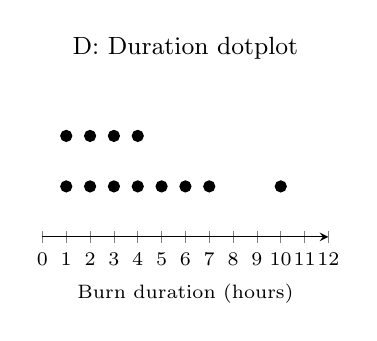
\begin{tikzpicture}\begin{axis}[width=0.43\linewidth,height=1.38in,xmin=0,xmax=12,ymin=0,ymax=3,xtick={0,1,...,12},ytick=\empty,axis y line=none,axis x line=bottom,xlabel={Burn duration (hours)},title={D: Duration dotplot},tick label style={font=\scriptsize},label style={font=\scriptsize},title style={font=\small}]
\addplot[only marks,mark=*,mark size=2pt] coordinates {(1,1) (1,2) (2,1) (2,2) (3,1) (3,2) (4,1) (4,2) (5,1) (6,1) (7,1) (10,1)};
\end{axis}\end{tikzpicture}
\end{tabular}
\end{center}
\begin{firsttakebox}{FIRST TAKE --- one sentence before you work the parts}
Which part of the proposed report needs the closest check, and why?
\workspace{0.25in}
\end{firsttakebox}

\begin{callout}{\IconBook\ Notes on Reading Displays}{calloutgreen}
Categorical variables record labels; quantitative variables record numerical amounts with units. A distribution describes values and their frequencies. Relative frequency is count divided by total; multiply by 100 for percent.\par A bar chart compares categories. A histogram groups measurements into intervals (bins); its height counts observations in each interval. A dotplot places one dot at each recorded value, stacking repeated values. A claim about an exact value needs evidence at that precision.
\end{callout}

\newpage
\textbf{Work (a)--(d).}\par\smallskip

\dokbadge{1}~\textbf{(a)} Name the categorical variable in A and give one of its categories. Name the quantitative variable in C and its unit.\par
\workspace{0.25in}

\dokbadge{2}~\textbf{(b)} Convert each count in A to a percent and compare with B. Explain whether these graphs represent different category distributions. \textbf{Check your response:} \fbox{\rule{0pt}{0.65em}\hspace{0.65em}} all three categories; \fbox{\rule{0pt}{0.65em}\hspace{0.65em}} total used; \fbox{\rule{0pt}{0.65em}\hspace{0.65em}} axis units.\par
\workspace{0.35in}

\dokbadge{2}~\textbf{(c)} Compare what the bar from 4 to 8 in C tells you with the dots over that interval in D. State the interval count and every individual duration there, including repeats. Explain the difference in precision, using candles and hours.\par
\workspace{0.35in}

\dokbadge{3}~\textbf{(d)} $\star$ Evaluate the editor\textquotesingle s plan in a short paragraph. Defend a set of displays sufficient for both reporting questions and correct any unsupported claims using numerical evidence. The teacher scores this response E/P/I by hand; nothing is automatically scored.\par
{\small\textbf{To earn an E, your answer must do ALL of these} (some = P; one or none = I):
\begin{itemize}[leftmargin=1.6em,itemsep=0pt,topsep=1pt,parsep=0pt]
  \item[{\setlength{\fboxsep}{0pt}\fbox{\rule{0pt}{0.65em}\hspace{0.65em}}}] Compare the wax categories and distributions in A and B using a numerical conversion and axis units.
  \item[{\setlength{\fboxsep}{0pt}\fbox{\rule{0pt}{0.65em}\hspace{0.65em}}}] Explain what the relevant histogram interval establishes and whether it supports the exact-duration claim.
  \item[{\setlength{\fboxsep}{0pt}\fbox{\rule{0pt}{0.65em}\hspace{0.65em}}}] Explain how the dotplot represents individual measurements and use it to check the exact-duration count with units.
  \item[{\setlength{\fboxsep}{0pt}\fbox{\rule{0pt}{0.65em}\hspace{0.65em}}}] Defend a sufficient set of displays for both workshop questions and state the resulting answers in context.
\end{itemize}}
\workspace{0.85in}

\begin{sentenceframebox}\raggedright\textbf{Frame:} For wax type, I would keep \blankt[0.6in]{display}; its axis uses \blankt[0.9in]{term}. For exact duration, I would keep \blankt[0.6in]{display} because it shows \blankt[1.1in]{term}.\end{sentenceframebox}

\begin{wordbankbox}\raggedright
\textbf{Word bank:} individual values \ensuremath{\;\cdot\;} C \ensuremath{\;\cdot\;} intervals \ensuremath{\;\cdot\;} counts \ensuremath{\;\cdot\;} category averages \ensuremath{\;\cdot\;} D \ensuremath{\;\cdot\;} A \ensuremath{\;\cdot\;} B \ensuremath{\;\cdot\;} percents \ensuremath{\;\cdot\;} cumulative totals
\par\smallskip{\footnotesize\color{framegray} Some words are not needed.}
\end{wordbankbox}

\textbf{Turn this sheet in whenever you finish --- bonus credit. Part (d) is scored E / P / I.}\par

\end{document}
